
\newcommand*{\Scale}[2][4]{\scalebox{#1}{$#2$}}%

\begin{frame}[fragile]{Sobre la noción de máquina}

	\[ \Scale[1.5]{ \text{Robots} \subset \text{Máquinas} }\] 
	
	\pause
	
	\[ \Scale[1.5]{\text{Autómatas} \subset \text{Máquinas} 	}\]
	
	\pause
	
	\[ \Scale[1.3]{\text{¿ Autómatas } \subset \text{Robots ?} } \quad \Scale[1.3]{\text{¿ Robots } \subset \text{Autómatas ?}}	\]
	
	\[ \Scale[1.5]{ \text{¿!Robots} = \text{Autómatas!?}}  \]

\end{frame}


\begin{frame}[fragile]{La ciencia de la máquina}

-Simple machine, any of several devices with few or no moving parts that are used to modify
motion and force in order to perform work. (Enciclopedia Britannica)

\vspace{10px}
\pause
\metroset{block=fill}
\begin{block}{Ladislao Retti: ’The Unknown Leonardo’}
	\begin{itemize}
		\pause
		\item - ’Thus Leonardo was the first to advocate the necessity of a science of mechanisms.’ -

		\pause
		
		\item - ’ A book about the nature of mechanism must precede a book about their aplications’ S. XVI

	\end{itemize}
\end{block}

\end{frame}

\begin{frame}[fragile]{Conceptualización de la máquina y el autómata}

\begin{itemize}
	\item Isaac Newton \quad  (25 de diciembre de 1642 - 20 de marzo 1727)
	\item Renee Descartes \quad  ( 31 de marzo 1596 - 11 de febrero 1650)
\end{itemize}

\vspace{10px}
\pause
\metroset{block=fill}
\begin{block}{El discurso del método 1637 }
	\begin{itemize}
		\pause
		\item - Es cosa digna de reflexión que aunque muchos animales muestran mayor habilidad que nosotros en algunas de sus acciones, en cambio son completamente ineptos para otras, de lo cual se infiere, no que tengan entendimiento [...] sólo la naturaleza guía sus actos según la disposición de sus órganos, a la manera que un reloj, compuesto solamente de ruedas y resortes.
		
		
	\end{itemize}
\end{block}

\end{frame}


\begin{frame}[fragile]{Conceptualización de la máquina y el autómata.}

	\begin{itemize}
		\item George Boole ( 2 de noviembre de 1815 - 	8 de diciembre de 1864)
	\end{itemize}
		
	\begin{columns}
		\begin{column}{0.5\textwidth}
			\vspace{10px}
			\pause
			\metroset{block=fill}
			\begin{block}{Sistemas Combinacionales }	
				\pause			
				 - Todo sistema digital en el que sus salidas son función exclusiva del valor de sus entradas en un momento dado, sin que intervengan en ningún caso estados anteriores de las entradas o de las salidas - 
					
				
			\end{block}
		\end{column}
		\begin{column}{0.5\textwidth}
			\pause
			\begin{figure}
				\centering
				
				\includegraphics[width=0.8\textwidth]{Automatas/Automatas}
				\caption{\href{https://es.wikipedia.org/wiki/Aut\%C3\%B3mata_finito}{link}}	
		\end{figure}
		\end{column}
	\end{columns}
		

\end{frame}


\begin{frame}[fragile]{Teoría de autómatas ( S. XX )}

	\begin{itemize}
		\item Alonzo Church - Cáculo lambda - ( 14 de junio 1903 – 11 de agosto 1995 )
		\item Stephen Kleene - Clausura de Kleene - (  5 de enero de 1909 - 25 de enero de 1994 )
		\item  Emil Leon Post - Máquina de Post - (11 de febrero de 1897  - 21 de abril de 1954 )
		\item Alan Turing  - Maquina de Turing - ( 23 de junio de 1912- 7 de junio de 1954 )
	\end{itemize}


\end{frame}

\begin{frame}[fragile]{Autómatas finitos}

\metroset{block=fill}
\begin{block}{ }
	\begin{itemize}
		\pause
		\item -  En electrónica un autómata es un sistema secuencial, aunque en ocasiones la palabra es
		utilizada también para referirse a un robot. [...] Sin embargo, la rápida evolución de los autómatas hace que esta definición no esté cerrada. (Wikipedia) -
	\end{itemize}
\end{block}
\pause 
Un autómata  es una tupla de 5 elementos: $(Q, \mathcal{A}, q_0, \delta, F)$

\begin{itemize}
	\item $Q$ : Conjunto finito de estados que numeramos $ q_0 \dots q_n$ \pause
	\item $\mathcal{A}$: Alfabeto, conjunto finito de símbolos sobre el que se crearán palabras del lenguaje. \pause
	\item $q_0$ El estado inicial. \pause
	\item $\delta :Q\times \mathcal{A} \rightarrow Q$. Función que nos indica cómo leer la palabra. \pause
	\item $F$ : Conjunto de estados finales
\end{itemize}


\end{frame}


\begin{frame}[fragile]{Ejemplos}

	\begin{figure}[h!]
		\centering
			
		\includegraphics[width=0.4\textwidth]{Automatas/pascalina}
		\caption{Sistema combinacional}	
		\end{figure}
	
	\pause
		\begin{figure}
			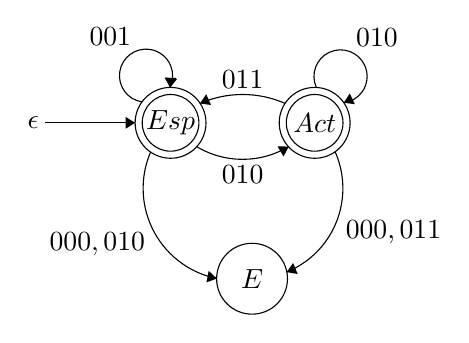
\begin{tikzpicture}[scale=0.15]
			\tikzstyle{every node}+=[inner sep=0pt]
			\draw [black] (37,-18.6) circle (3);
			\draw (37,-18.6) node {$Esp$};
			\draw [black] (37,-18.6) circle (2.4);
			\draw [black] (49.2,-18.6) circle (3);
			\draw (49.2,-18.6) node {$Act$};
			\draw [black] (49.2,-18.6) circle (2.4);
			\draw [black] (43.9,-31.8) circle (3);
			\draw (43.9,-31.8) node {$E$};
			\draw [black] (39.494,-16.958) arc (113.75402:66.24598:8.952);
			\fill [black] (39.49,-16.96) -- (40.43,-17.09) -- (40.02,-16.18);
			\draw (43.1,-15.7) node [above] {$011$};
			\draw [black] (46.998,-20.609) arc (-58.98762:-121.01238:7.566);
			\fill [black] (47,-20.61) -- (46.05,-20.59) -- (46.57,-21.45);
			\draw (43.1,-22.19) node [below] {$010$};
			\draw [black] (37,-15.5) -- (37,-15.6);
			\fill [black] (37,-15.6) -- (37.5,-14.8) -- (36.5,-14.8);
			\draw [black] (34.59,-16.833) arc (261.47443:-26.52557:2.25);
			\draw (31.9,-12.1) node [above] {$001$};
			\fill [black] (36.94,-15.61) -- (37.55,-14.9) -- (36.56,-14.75);
			\draw [black] (26.4,-18.6) -- (34,-18.6);
			\draw (25.9,-18.6) node [left] {$\epsilon$};
			\fill [black] (34,-18.6) -- (33.2,-18.1) -- (33.2,-19.1);
			\draw [black] (50.924,-21.032) arc (24.0977:-67.85012:7.646);
			\fill [black] (46.83,-31.24) -- (47.76,-31.4) -- (47.38,-30.47);
			\draw (51.79,-27.89) node [right] {${000,011}$};
			\draw [black] (40.919,-31.779) arc (-101.43921:-203.36619:7.786);
			\fill [black] (40.92,-31.78) -- (40.23,-31.13) -- (40.04,-32.11);
			\draw (34.88,-28.9) node [left] {${000,010}$};
			\draw [black] (49.35,-15.615) arc (204.86229:-83.13771:2.25);
			\draw (54.48,-12.2) node [above] {$010$};
			\fill [black] (51.66,-16.9) -- (52.6,-17.02) -- (52.18,-16.11);
			
			\end{tikzpicture}
			\caption{Automata finito}
		\end{figure}

\end{frame}


\begin{frame}[fragile]{Máquina de Turing}

		\begin{columns}
		\begin{column}{0.5\textwidth}
			\begin{itemize}
				\item $Q$  Conjunto finito de estados
				\item $A$  Alfabeto de entrada
				\item $B$  Alfabeto de símbolos en la cinta , $A\subset B$
				\item $\delta$ Función de transición
				\item $q_0$ Estado inicial
				\item $\# \in B-A$ El 'símbolo blanco'
				\item $F$ Conjunto de estados finales
			\end{itemize}
		\end{column}
		\begin{column}{0.5\textwidth}
			\pause
			\begin{figure}
				\centering
				
				\includegraphics[width=\textwidth]{Automatas/turingMahchine}
				\caption{\href{https://es.wikipedia.org/wiki/Aut\%C3\%B3mata_finito}{MT}}	
			\end{figure}
		\end{column}
	\end{columns}
	
\end{frame}


\begin{frame}[fragile]{Turing Completitud }

\metroset{block=fill}
\begin{block}{Máquina de Turing Universales}
	\begin{itemize}
		\pause
		\item -   Máquina de Turing que puede simular una máquina de Turing arbitraria en la entrada arbitraria. -
	\end{itemize}


\end{block}
\pause
\begin{block}{Casualmente Turing Completo: El juego de la vida }

	\begin{itemize}
		\item Una casilla con exactamente 3 vecinas 'vivas' nace.
		\item Una casilla con 2 o 3 vecinas vivas sigue viva, en otro caso muere.
	\end{itemize}
	
\end{block}

\end{frame}

\begin{frame}[fragile]{Inteligencia Artificial }

\metroset{block=fill}
\begin{block}{Inteligencia débil vs Inteligencia fuerte }
	
	\begin{itemize}
		\item 'La inteligencia artificial está relacionada con conductas inteligentes en artefactos' (Nilsson,1998).
		\pause
		\item 'El nuevo y excitante esfuerzo de hacer que los computadores piensen...,máquinas con mentes, en el sentido más literal' (Haugeland,1985).
	\end{itemize}
	
\end{block}

\end{frame}

\begin{frame}[fragile]{¿Pueden pensar las máquinas ?}

\begin{columns}
	\begin{column}{0.5\textwidth}
		\begin{figure}
			\centering
			
			\includegraphics[width=\textwidth]{Automatas/turing_test}
			\caption{\href{https://es.wikipedia.org/wiki/Aut\%C3\%B3mata_finito}{Test de Turing}}	
				
		\end{figure}
		
	\end{column}
	\begin{column}{0.5\textwidth}
		\pause
		\begin{figure}
			\centering
			
			\includegraphics[width=\textwidth]{Automatas/descarga}
			\caption{\href{https://horaciobacon.wordpress.com/2017/06/29/el-extrano-caso-de-la-habitacion-china/}{Habitación China}}
		\end{figure}
	\end{column}
\end{columns}

\end{frame}


\begin{frame}[fragile]{}

\metroset{block=fill}
\begin{block}{Alan Turing (1950) }
	
	\begin{itemize}
		\item  ’Solo podemos prever el futuro inmediato, pero de lo
		que cabe duda es de que hay mucho por hacer’.
	\end{itemize}
	
\end{block}

\end{frame}

%\vspace{10px}
%\pause
%\metroset{block=fill}
%\begin{block}{}
%	\begin{itemize}
%		\item Arquitas de Tarento
%		\pause
%		\item Apolonio de Pérgamo
%		\pause
%		\item Ctesibio de Alejandría
%		\pause
%		\item Filón de Bizancio
%		\pause
%		\item Herón de Alejandría
%		\pause
%		\item Alejandro Magno
%	\end{itemize}
%\end{block}